% structure as seen in https://www.overleaf.com/learn/latex/How_to_Write_a_Thesis_in_LaTeX_(Part_1):_Basic_Structure

\documentclass[12pt]{report}
\usepackage[utf8]{inputenc}
\usepackage{graphicx}
\usepackage{amsmath}
\usepackage{amssymb}
\graphicspath{ {images/} }
\usepackage[ruled,vlined]{algorithm2e}

\usepackage{amsthm}

\theoremstyle{definition}
\newtheorem{definition}{Definition}[section]

\title{
{Separation of Foreground and Background Signal in Variational Autoencoders}\\
{\large Albert-Ludwigs-Universität Freiburg}\\[\baselineskip]
{
\includegraphics[width=7cm]{logo.png}}
}
\author{Florian Eichin}
\date{02.12.1995}

\begin{document}

\maketitle

\leavevmode\thispagestyle{empty}\newpage

\begin{center}
\vspace*{\fill}
\emph{Meiner Familie.}
\vspace*{\fill}
\end{center}

\leavevmode\thispagestyle{empty}\newpage

\leavevmode\thispagestyle{empty}\newpage

\chapter*{Declaration}
I hereby declare that the thesis submitted is my own unaided work. All direct or indirect sources used are acknowledged as references. This work was not previously presented to another examination board and has not been published. \\ \\ \\ \\ \\

Freiburg, \today



\tableofcontents

\chapter{Introduction}
With the rise of computation power in the last decades, Machine Learning approaches have revolutionized the algorithmic solving of various practical problems, that were deemed unlikely to be tackled successfully for a long time. Simultaneously, the data we collect about the world becomes more detailed than ever before. With datasets of hundreds of gigabytes, Artificial Neural Networks, a family of algorithms, that profits from both, big data and computation power, are being applied to all kinds of domains and have replaced many state-of-the-art approaches or at least matched their performance.

This work is motivated by the use-case of separating foreground and background signal within image data. Take for example an image taken by your camera: Usually there are parts of the image, that are within focus and appear sharp on the photography. We refer to this as foreground of the image. The foreground usually contains most of the informative parts, like, for example, your face or cat (or both). Parts, that are out of focus, appear more blurry and usually span over large partitions of the image. With the same logic, these components are called background. The background contains the less informative parts, like for example trees or your couch, which were not object of the photography. In the examples given, it is usually not hard for a human to seperate foreground and background. However, even with this kind of data, it is hard to teach this as an procedure to a computer. In this case, we can use human experts to label images and use machine learning algorithms, that work in a supervised manner. But what if we have image data, where even the best trained humans are not able to discriminate between back- and foreground in an efficient way? To give an example, we are often confronted with this problem in medical image data, which is the main motivation for this work. To be more precise, the starting point of this thesis was video data, obtained from a technique called 2-photon excitation microscopy. It contains information about the activity of neural cells within the brain of a mouse. In this case, we want to separate the activity of neural cells in the focussed foreground from the activity of cells, that were not within focus of the images. Human experts are usually not able to label large amounts of such data correctly and efficiently, which is why unsupervised machine learning approaches are needed.

In this work, the Variational Autoencoder, a statistical latent variable model, that was introduced by Kingma and Welling in \cite{kingma2} and is an example for an application of Artificial Neural Networks, will be derived and evaluated on artificial datasets, that resemble the scenario described above. First, a theoretical background will be built by introducing latent variable models and variational inference. In the following, a target, known as the Variational Lower Bound or ELBO, will be derived as well as an approach to optimize it, the Auto-encoding Variational Bayes algorithm. Subsequently, we will introduce the Variational Autoencoder and discuss Neural Networks as a way to parameterize the model. Concluding the theoretical part, Convolutional Neural Networks and a special double-ELBO structure for our problem setup will be described.
In the second part of this thesis, we will specify the datasets and the implementation of the algorithm. Subsequently, the results of the evaluation of the separative ability will be described and discussed.

\chapter{Theoretical Part}

In the following, the necessary theoretical background to derive the Variational Autoencoder (VAE) model is introduced. Adding to that, we will describe a possible extension of classical VAEs for the purpose of separating background and foreground signal in image data.
The following sections mainly follows the arguments presented in \cite{kingma1}. Also, \cite{kingma2} and \cite{stanford} provided ideas that have been incorporated. As for notation, we use lower case bolt letters (e.g. $\mathbf{x}$) to denote a vector of random variables and uppercase bolt letters (e.g. $\mathbf{X} = \{ \mathbf{x}^{(1)}, ..., \mathbf{x}^{(n)}\}$) to denote sets of such random variables, which will also be called \emph{datasets}.

\section{Inference Problem}
Before diving into the technical questions of this thesis, let us begin with a discussion of the problem we attempt to solve. Let $\mathbf{x}, \mathbf{z}$ be random variables with $\mathbf{x}$ observable and $\mathbf{z}$ hidden. Then we are interested in the \textit{latent variable model} with model parameters $\pmb{\theta}^*$
\begin{equation}
	p_{\pmb{\theta}^*}(\mathbf{x}, \mathbf{z}) = p_{\pmb{\theta}^*}(\mathbf{x}| \mathbf{z})p_{\pmb{\theta}^*}(\mathbf{z})
\end{equation}
Furthermore, it is assumed that prior $p_{\pmb{\theta}^*}(\mathbf{z})$ and $p_{\pmb{\theta}^*}(\mathbf{x}|\mathbf{z})$ are from parametric families of distributions $(p_{\pmb{\theta}}(\mathbf{z}))_{\pmb{\theta} \in \pmb{\Theta}}$ and $(p_{\pmb{\theta}}(\mathbf{x}|\mathbf{z}))_{\pmb{\theta} \in \pmb{\Theta}}$ and that they have probability density functions, that are differentiable with respect to $\pmb{\theta}$ and $\mathbf{z}$ almost everywhere.

Clearing things by looking at it in a more practical way: Let $\mathbf{X} = \{ \mathbf{x}^{(i)}\}_{i=1}^N$ be a dataset with $N \in \mathbb{N}$ i.i.d. samples of our random variable $\mathbf{x}$. Note, that $\mathbf{x}$ can be a vector of arbitrary dimension encoding all kinds of data such as images, soundwaves etc. Moddeling the data with the above latent variable model, the datapoints $\mathbf{x}^{(i)}$ are supposed to be generated with the involvement of $\mathbf{z}$ in the sense, that first a value $\mathbf{z}^{(i)}$ is generated from prior distribution $p_{\mathbf{\theta^*}}(\mathbf{z})$ and in the second step, $\mathbf{x}^{(i)}$ is generated from $p_{\pmb{\theta}^*}(\mathbf{x}|\mathbf{z}^{(i)})$.
Usually, $\mathbf{z}$ is assumed to have a much lower dimension and a simpler distribution than $\mathbf{x}$. Therefore, the $\mathbf{z}$-space can be viewed as a space of encodings, where only relevant information for decoding datapoints into the high-dimensional $\mathbf{x}$-space is retained. This is why, from a machine learning perspective, we can view the problem of finding optimal parameters $\pmb{\theta}^*$ as a dimensionality reduction problem.
For a given dataset, there are different approaches for the this scenario. However, we do make additional assumptions, that narrow the list of efficient algorithms significantly according to \cite{kingma1}.

\begin{itemize}
	\item[1] \emph{Intractability}: the marginal likelihood $p_{\pmb{\theta}}(\mathbf{x}) = \int p_{\pmb{\theta}}(\mathbf{z}) p_{\pmb{\theta}}(\mathbf{x}|\mathbf{z}) d \mathbf{z}$, as well as posterior distribution $p_{\pmb{\theta}}(\mathbf{z}|\mathbf{x}) = p_{\pmb{\theta}}(\mathbf{x}|\mathbf{z}) p_{\pmb{\theta}}(\mathbf{z}) / p_{\pmb{\theta}}(\mathbf{x})$ are intractable.
	\item[2] \emph{Big dataset}: Optimization on the whole dataset is too expensive and parameter updates on small minibatches (see 2.5.3) preferable. Sampling-based solutions would be too inefficient according to \cite{kingma1}.
\end{itemize}

\section{Variational Inference}
In many probabilistic models, inference is intractable and approximation methods are needed. One way of approximating solutions to inference problems, is to describe it as an optimization problem over a family of tractable distributions. Algorithms involving this approach are called \emph{variational}.
Given an intractable probability distribution $p$ and a family of tractable distributions $(q_{\pmb{\phi}})_{\pmb{\phi} \in \pmb{\Phi}}$, the goal of a variational algorithm, is to find $\pmb{\phi} \in \pmb{\Phi}$ such that $q_{\pmb{\phi}}$ is most 'similar' to $p$. Finding such parameters $\pmb{\phi}$ usually involves a complex optimization procedure for an optimization target $\mathcal{L}_{\pmb{\phi}}$. Subsequently, we can use $q_{\pmb{\phi}}$ instead of $p$ in order to find approximate solutions to inference problems efficiently.\\
Of course, this description of variational techniques leaves us with questions. What is the similarity of two distributions $q_{\pmb{\phi}}$ and $p_{\pmb{\theta}}$? How is an according optimization objective $\mathcal{L}_{\pmb{\phi}}$ chosen? What is a good way of formulating the tractable family of distributions $(q_{\pmb{\phi}})_{\pmb{\phi} \in \pmb{\Phi}}$? \\
The (partial) answering to these three questions for the latent variable model, described in the previous section, will be the main motivation for the following sections in order to lay the groundwork for the introduction of the Variational Autoencoder (VAE). Inheriting it's name from \emph{Autoencoders}[XX], a VAE is a probabilistic model designed for learning latent representations with the help of Artificial Neuronal Networks (ANNs) and a variational optimization approach to the approximation of the encoder distribution.

\section{Kullback-Leibler Divergence}
Beginning with the first question, there is a way of quantifying the 'similarity' of two distributions $p(\mathbf{x})$ and $q(\mathbf{x})$ in information theory, known as the \emph{Kullback-Leibler (KL) divergence}. For $p(\mathbf{x}), q(\mathbf{x})$ continuous, the KL divergence is defined as:
\begin{equation}
	KL(q(\mathbf{x})||p(\mathbf{x})) := \int_{-\infty}^{\infty} q(\mathbf{x}) \log \frac{q(\mathbf{x})}{p(\mathbf{x})} d \mathbf{x}
\end{equation}
In the discrete case, it is
\begin{equation}
	KL(q(\mathbf{x})||p(\mathbf{x})) := \sum_{\mathbf{x}} q(\mathbf{x}) \log \frac{q(\mathbf{x})}{p(\mathbf{x})}
\end{equation}
Here, $\log$ is an abbreviation for the logarithm to base $e$, the natural logarithm. Note, that for any $q(\mathbf{x}), p(\mathbf{x})$ (continuous or discrete) we can deduce $KL(q||p) \geq 0$.
Consider $q(\mathbf{x}), p(\mathbf{x})$ to be continuous (the discrete case follows analogously). With $1 - r \leq -\log(r)$ we have:
\begin{equation}
\begin{split}
KL(q(\mathbf{x})||p(\mathbf{x}))
& = \int_{\mathbf{x}} q(\mathbf{x}) \log \frac{q(\mathbf{x})}{p(\mathbf{x})} d \mathbf{x} \\
& = \int_{\mathbf{x}} q(\mathbf{x}) (- \log \frac{p(\mathbf{x})}{q(\mathbf{x})}) d \mathbf{x} \\
& \geq \int_{\mathbf{x}} q(\mathbf{x}) (1 - \frac{p(\mathbf{x})}{q(\mathbf{x})}) d \mathbf{x} \\
& = \int_{\mathbf{x}} q(\mathbf{x}) d \mathbf{x} - \int_{\mathbf{x}} q(\mathbf{x}) \frac{p(\mathbf{x})}{q(\mathbf{x})} d \mathbf{x} = 0
\end{split}
\end{equation}
Also, the KL divergence can be rewritten in both cases as an expectation:
\begin{equation}
	KL(q(\mathbf{x})||p(\mathbf{x})) = \mathbb{E}_{q(\mathbf{x})}\left[ \log\left(\frac{q(\mathbf{x})}{p(\mathbf{x})} \right) \right]
\end{equation}

\section{Variational Lower Bound (ELBO)}
As discussed previously, $p_{\pmb{\theta}}(\mathbf{x})$ as well as $p_{\pmb{\theta}}(\mathbf{z}|\mathbf{x})$ are intractable in the given problem setup. There is thus no way of retrieving either of the two out of the other. This is where variational approximation from two sections before can be used. In order to approximate $p_{\pmb{\theta}}(\mathbf{z}|\mathbf{x})$ we introduce a tractable inference model $q_{\pmb{\phi}}(\mathbf{z}|\mathbf{x})$ with parameters $\pmb{\phi}$. In the following, we sometimes will refer to $p_{\pmb{\theta}}(\mathbf{z}|\mathbf{x})$ as \emph{decoder distribution} or just \emph{decoder} and to $q_{\pmb{\phi}}(\mathbf{z}|\mathbf{x})$ as \emph{encoder}. Being a variational approach,  $\pmb{\phi}$ will be optimized such that $p_{\pmb{\theta}}(\mathbf{z}|\mathbf{x})$ is most similar to $q_{\pmb{\phi}}(\mathbf{z}|\mathbf{x})$ with respect to KL divergence.
Derived from Bayes' rule, we also have:
\begin{equation}
	p_{\pmb{\theta}}(\mathbf{x}) = \frac{p_{\pmb{\theta}}(\mathbf{z}|\mathbf{x}) p_{\pmb{\theta}}(\mathbf{z})}{p_{\pmb{\theta}}(\mathbf{x}|\mathbf{z})} \approx  \frac{p_{\pmb{\theta}}(\mathbf{z}|\mathbf{x}) p_{\pmb{\theta}}(\mathbf{z})}{q_{\pmb{\phi}}(\mathbf{x}|\mathbf{z})}
\end{equation}
It is clear, in order for our model to fit the true distribution of our data, we are interested in the following two things:
\begin{itemize}
	\item[1.] Maximization of the marginal likelihood $p_{\pmb{\theta}}(\mathbf{x})$ for the data to improve the generative model.
	\item[2.] Minimization of the KL divergence between $q_{\pmb{\phi}}(\mathbf{z}|\mathbf{x})$ and $p_{\pmb{\theta}}(\mathbf{z}|\mathbf{x})$ to improve the approximation of $q_{\pmb{\phi}}(\mathbf{z}|\mathbf{x})$.
\end{itemize}
Since $\log$ is monotonous, maximizing $p_{\pmb{\theta}}(\mathbf{x})$ is equivalent to maximizing $\log p_{\pmb{\theta}}(\mathbf{x})$. For an arbitrary choice of $q_{\pmb{\phi}}(\mathbf{z}|\mathbf{x})$ consider the following derivation:
\begin{equation}
\begin{split}
	\log p_{\pmb{\theta}}(\mathbf{x})
	& = \mathbb{E}_{q_{\pmb{\phi}}(\mathbf{z}|\mathbf{x})}\left[\log p_{\pmb{\theta}}(\mathbf{x})\right] \\
	& = \mathbb{E}_{q_{\pmb{\phi}}(\mathbf{z}|\mathbf{x})}\left[ \log \frac{p_{\pmb{\theta}}(\mathbf{x}, \mathbf{z})}{p_{\pmb{\theta}}(\mathbf{z}|\mathbf{x})} \right] \\
	& = \mathbb{E}_{q_{\pmb{\phi}}(\mathbf{z}|\mathbf{x})}\left[ \log\left(\frac{p_{\pmb{\theta}}(\mathbf{x}, \mathbf{z})}{q_{\pmb{\phi}}(\mathbf{z}|\mathbf{x})}\frac{q_{\pmb{\phi}}(\mathbf{z}|\mathbf{x})}{p_{\pmb{\theta}}(\mathbf{z}|\mathbf{x})} \right) \right] \\
	& = \mathbb{E}_{q_{\pmb{\phi}}(\mathbf{z}|\mathbf{x})}\left[ \log\left(\frac{p_{\pmb{\theta}}(\mathbf{x}, \mathbf{z})}{q_{\pmb{\phi}}(\mathbf{z}|\mathbf{x})}\right) \right] + \mathbb{E}_{q_{\pmb{\phi}}(\mathbf{z}|\mathbf{x})}\left[ \log\left(\frac{q_{\pmb{\phi}}(\mathbf{z}|\mathbf{x})}{p_{\pmb{\theta}}(\mathbf{z}|\mathbf{x})} \right) \right] \\
	& = \mathbb{E}_{q_{\pmb{\phi}}(\mathbf{z}|\mathbf{x})}\left[ \log\left(\frac{p_{\pmb{\theta}}(\mathbf{x}, \mathbf{z})}{q_{\pmb{\phi}}(\mathbf{z}|\mathbf{x})}\right) \right] + KL(q_{\pmb{\phi}}(\mathbf{z}|\mathbf{x}) || p_{\pmb{\theta}}(\mathbf{z}| \mathbf{x}))
\end{split}
\end{equation}
Where the right term in the last row is the KL divergence of $q_{\pmb{\phi}}(\mathbf{z}|\mathbf{x})$ and $p_{\pmb{\theta}}(\mathbf{x}, \mathbf{z})$. If we rearrange the equation, we have the following:
\begin{equation}
	\log p_{\pmb{\theta}}(\mathbf{x}) - KL(q_{\pmb{\phi}}(\mathbf{z}|\mathbf{x}) || p_{\pmb{\theta}}(\mathbf{z}| \mathbf{x})) = \mathbb{E}_{q_{\pmb{\phi}}(\mathbf{z}|\mathbf{x})}\left[ \log\left(\frac{p_{\pmb{\theta}}(\mathbf{x}, \mathbf{z})}{q_{\pmb{\phi}}(\mathbf{z}|\mathbf{x})}\right) \right]
\end{equation}
And since $KL(q_{\pmb{\phi}}(\mathbf{z}|\mathbf{x}) || p_{\pmb{\theta}}(\mathbf{x}, \mathbf{z})) \geq 0$, the right hand side is a lower bound for $\log p_{\pmb{\theta}}(\mathbf{x})$. It is also referred to as \emph{variational lower bound} or \emph{evidence lower bound} (ELBO):
\begin{equation}
\begin{split}
	\mathcal{L}_{\pmb{\theta}, \pmb{\phi}}(\mathbf{x})
	& = \mathbb{E}_{q_{\pmb{\phi}}(\mathbf{z}|\mathbf{x})}\left[ \log\left(\frac{p_{\pmb{\theta}}(\mathbf{x}, \mathbf{z})}{q_{\pmb{\phi}}(\mathbf{z}|\mathbf{x})}\right) \right] \\
	& = \mathbb{E}_{q_{\pmb{\phi}}(\mathbf{z}|\mathbf{x})}\left[ \log p_{\pmb{\theta}}(\mathbf{x}, \mathbf{z}) - \log q_{\pmb{\phi}}(\mathbf{z}|\mathbf{x}) \right] \\\\
\end{split}
\end{equation}
We will keep this form of the ELBO for the rest of this work, however it can be rewritten in the following way (leading to different estimators in other literature, for example \cite{kingma2}):
\begin{equation}
\begin{split}
& \mathbb{E}_{q_{\pmb{\phi}}(\mathbf{z}|\mathbf{x})}\left[ \log\left(\frac{p_{\pmb{\theta}}(\mathbf{x}, \mathbf{z})}{q_{\pmb{\phi}}(\mathbf{z}|\mathbf{x})}\right) \right] \\
& = \mathbb{E}_{q_{\pmb{\phi}}(\mathbf{z}|\mathbf{x})}\left[ \log\left(\frac{p_{\pmb{\theta}}(\mathbf{x}|\mathbf{z})p_{\pmb{\theta}}(\mathbf{z})}{q_{\pmb{\phi}}(\mathbf{z}|\mathbf{x})}\right) \right] \\
	& = \mathbb{E}_{q_{\pmb{\phi}}(\mathbf{z}|\mathbf{x})}\left[ \log p_{\pmb{\theta}}(\mathbf{x}| \mathbf{z}) - \log \frac{q_{\pmb{\phi}}(\mathbf{z}|\mathbf{x})}{p_{\pmb{\theta}}(\mathbf{z})} \right]	\\
	& = \mathbb{E}_{q_{\pmb{\phi}}(\mathbf{z}|\mathbf{x})}\left[ \log p_{\pmb{\theta}}(\mathbf{x}| \mathbf{z})\right] - \mathbb{E}_{q_{\pmb{\phi}}(\mathbf{z}|\mathbf{x})}\left[\log \frac{q_{\pmb{\phi}}(\mathbf{z}|\mathbf{x})}{p_{\pmb{\theta}}(\mathbf{z})} \right]	\\
	& = \mathbb{E}_{q_{\pmb{\phi}}(\mathbf{z}|\mathbf{x})}\left[ \log p_{\pmb{\theta}}(\mathbf{x}| \mathbf{z})\right] + KL(q_{\pmb{\phi}}(\mathbf{z}|\mathbf{x})||p_{\pmb{\theta}}(\mathbf{z}))\\
\end{split}
\end{equation}
With the above derivation (2.7) in mind, one can identify another interpretation of $KL(q_{\pmb{\phi}}(\mathbf{z}|\mathbf{x}) || p_{\pmb{\theta}}(\mathbf{z}|\mathbf{x}))$ besides being the KL divergence of approximate posterior $q_{\pmb{\phi}}(\mathbf{z}|\mathbf{x})$ and true posterior $p_{\pmb{\theta}}(\mathbf{z}| \mathbf{x}))$: It is also the gap between ELBO $\mathcal{L}_{\pmb{\theta}, \pmb{\phi}}(\mathbf{x})$ and $\log p_{\pmb{\theta}}(\mathbf{x})$. If $q_{\pmb{\phi}}(\mathbf{z}|\mathbf{x})$ approximates the true $p_{\pmb{\theta}}(\mathbf{z}|\mathbf{x})$ 'better', the gap gets smaller.

Let $\mathbf{X}$ be the dataset of i.i.d. samples from before and $N_{\mathbf{X}} = |\mathbf{X}|$. If we want to fit our model on $\mathbf{X}$, the ELBO yields an optimization objective we were asking for, namely the average of ELBOs of single datapoints $\mathbf{x} \in \mathbf{X}$:
\begin{equation}
	\mathcal{L}_{\pmb{\theta}, \pmb{\phi}}(\mathbf{X}) = \sum_{\mathbf{x} \in \mathbf{X}} \frac{\mathcal{L}_{\pmb{\theta}, \pmb{\phi}}(\mathbf{x})}{N_{\mathbf{X}}}
\end{equation}
Maximizing $\mathcal{L}_{\pmb{\theta}, \pmb{\phi}}(\mathbf{x})$, with respect to parameters $\pmb{\theta}$ and $\pmb{\phi}$ for our data, will approximately maximize $p_{\pmb{\theta}}(\mathbf{x})$ and minimize $KL(q_{\pmb{\phi}}(\mathbf{z}|\mathbf{x}) || p_{\pmb{\theta}}(\mathbf{z}| \mathbf{x}))$, satisfying the goals formulated in the beginning of this section.

\section{Auto-encoding Variational Bayes}
\subsection{Batch Gradient Descent}
With the means of the ELBO, we now have an objective to optimize the model parameters $\pmb{\theta}$ and $\pmb{\phi}$ for. A naive solution, also known as \emph{Batch Gradient Descent}, is, to initialize the parameters randomly, to estimate the gradients $\nabla_{\pmb{\theta}}\mathcal{L}_{\pmb{\theta}, \pmb{\phi}}(\mathbf{X})$ and $\nabla_{\pmb{\pmb{\phi}}}\mathcal{L}_{\pmb{\theta}, \pmb{\phi}}(\mathbf{X})$ and adjust $\pmb{\theta}$ and $\pmb{\phi}$ into their respective directions until convergence. With each step of adjusting the parameters for the gradients, also called an \emph{epoch}, we expect $\mathcal{L}_{\pmb{\theta}, \pmb{\phi}}(\mathbf{X})$ to improve until we have reached a local maximum and the algorithm converges. It is up to implementation, how to detect convergence of the algorithm. Typically, one can define criteria such as a threshold for change of loss after a certain number of epochs. If the change of loss is lower than this set threshhold, we abort the procedure. Of course, there is other, more complex criteria. Sometimes the user decides themselves, when to stop the algorithm, due to the tradeoff between runtime and optimality.

\begin{algorithm}[H]
\SetAlgoLined
\While{not converged}{
Estimate gradients $\nabla_{\pmb{\theta}}\mathcal{L}_{\pmb{\theta}, \pmb{\phi}}(\mathbf{X})$, $\nabla_{\pmb{\pmb{\phi}}}\mathcal{L}_{\pmb{\theta}, \pmb{\phi}}(\mathbf{X})$\\
Update parameters $\pmb{\theta} \rightarrow \pmb{\theta} + \eta \nabla_{\pmb{\theta}}\mathcal{L}_{\pmb{\theta}, \pmb{\phi}}(\mathbf{X})$, $\pmb{\phi} \rightarrow \pmb{\phi} + \eta \nabla_{\pmb{\phi}}\mathcal{L}_{\pmb{\theta}, \pmb{\phi}}(\mathbf{X})$
}
\caption{Batch Gradient Descent}
\end{algorithm}
Note, that $\eta$ is a hyperparameter, that determines the extent, to which the gradients update the parameters in each epoch. It is therefore also called the \emph{learning rate} and is an important parameter to choose as it highly affects the convergence of the algorithm: If we choose $\eta$ too small, the algorithm will only move slowly into the 'preferred' direction of local maxima. However, if $\eta$ is chosen too big, the updating-steps get too large and the algorithm cannot converge in the worst case.


\subsection{Estimation of the Gradients and ELBO}
In general, analytical computations of the gradients of the ELBO are intractable, so they have to be estimated. For $\nabla_{\pmb{\theta}, \pmb{\phi}}\mathcal{L}_{\pmb{\theta}, \pmb{\phi}}(\mathbf{X})$, it is sufficient to estimate $\nabla_{\pmb{\theta}, \pmb{\phi}}\mathcal{L}_{\pmb{\theta}, \pmb{\phi}}(\mathbf{x})$ for each $\mathbf{x} \in \mathbf{X}$ because since (2.11) we have:
\begin{equation}
	\nabla_{\pmb{\theta}, \pmb{\phi}}\mathcal{L}_{\pmb{\theta}, \pmb{\phi}}(\mathbf{X}) = \nabla_{\pmb{\theta}, \pmb{\phi}}  \sum_{\mathbf{x} \in \mathbf{X}} \frac{\mathcal{L}_{\pmb{\theta}, \pmb{\phi}}(\mathbf{x})}{N_{\mathbf{X}}} = \frac{1}{N_{\mathbf{X}}} \sum_{\mathbf{x} \in \mathbf{X}} \nabla_{\pmb{\theta}, \pmb{\phi}} \mathcal{L}_{\pmb{\theta}, \pmb{\phi}}(\mathbf{x})
\end{equation}
For gradients of the ELBO with respect to generative model parameters $\pmb{\theta}$, we can obtain an unbiased Monte Carlo estimator (unbiased estimation will from now on be illustrated by '$\simeq$'):
\begin{equation}
\begin{split}
\nabla_{\pmb{\theta}}\mathcal{L}_{\pmb{\theta}, \pmb{\phi}}(\mathbf{x})
& \stackrel{(2.9)}{=} \nabla_{\pmb{\theta}} \mathbb{E}_{q_{\pmb{\phi}}(\mathbf{z}|\mathbf{x})}\left[ \log p_{\pmb{\theta}}(\mathbf{x}, \mathbf{z}) - \log q_{\pmb{\phi}}(\mathbf{z}|\mathbf{x}) \right]	\\
& = \mathbb{E}_{q_{\pmb{\phi}}(\mathbf{z}|\mathbf{x})}\left[ \nabla_{\pmb{\theta}} (\log p_{\pmb{\theta}}(\mathbf{x}, \mathbf{z}) - \log q_{\pmb{\phi}}(\mathbf{z}|\mathbf{x})) \right] \\
& \simeq \nabla_{\pmb{\theta}} (\log p_{\pmb{\theta}}(\mathbf{x}, \mathbf{z}) - \log q_{\pmb{\phi}}(\mathbf{z}|\mathbf{x})) \\
& = \nabla_{\pmb{\theta}} \log p_{\pmb{\theta}}(\mathbf{x}, \mathbf{z})\\
\end{split}
\end{equation}
With the $\mathbf{z}$ in the last two lines a random sample from $q_{\pmb{\phi}}(\mathbf{z}|\mathbf{x})$. For unbiased gradients with respect to $\pmb{\phi}$, things are a more difficult. This is due to the fact, that in general, we have:
\begin{equation}
\begin{split}
\nabla_{\pmb{\phi}}\mathcal{L}_{\pmb{\theta}, \pmb{\phi}}(\mathbf{x})
& = \nabla_{\pmb{\phi}} \mathbb{E}_{q_{\pmb{\phi}}(\mathbf{z}|\mathbf{x})}\left[ \log p_{\pmb{\theta}}(\mathbf{x}, \mathbf{z}) - \log q_{\pmb{\phi}}(\mathbf{z}|\mathbf{x}) \right]	\\
& \neq \mathbb{E}_{q_{\pmb{\phi}}(\mathbf{z}|\mathbf{x})}\left[ \nabla_{\pmb{\phi}} (\log p_{\pmb{\theta}}(\mathbf{x}, \mathbf{z}) - \log q_{\pmb{\phi}}(\mathbf{z}|\mathbf{x})) \right] \\
\end{split}
\end{equation}
Moreover, we will thus assume $\mathbf{z}$ to be continuous and $q_{\pmb{\phi}}(\mathbf{z}|\mathbf{x})$ and $p_{\pmb{\theta}}(\mathbf{x}|\mathbf{z})$ differentiable. For the case of the Variational Autoencoder (and other instances of our problem), this is not much of a constraint. However, we can now reparameterize $\mathbf{z} \sim q_{\pmb{\phi}}(\mathbf{z}|\mathbf{x})$ to circumvent the problem of obtaining $\nabla_{\pmb{\phi}}\mathcal{L}_{\pmb{\theta}, \pmb{\phi}}(\mathbf{x})$. We can choose $f$ as some invertible, differentiable transformation and introduce another random variable $\pmb{\epsilon} \sim p(\pmb{\epsilon})$ independent of $\pmb{\phi}$, $\pmb{\theta}$ and $\mathbf{x}$ such that:
\begin{equation}
\mathbf{z} = f(\pmb{\epsilon}, \pmb{\phi}, \mathbf{x})
\end{equation}
This is also referred to as \emph{reparameterization trick}. Under reparameterization, the ELBO can be rewritten and estimated:
\begin{equation}
\begin{split}
\mathcal{L}_{\pmb{\theta}, \pmb{\phi}}(\mathbf{x})
& = \mathbb{E}_{q_{\pmb{\phi}}(\mathbf{z}|\mathbf{x})}\left[ \log p_{\pmb{\theta}}(\mathbf{x}, \mathbf{z}) - \log q_{\pmb{\phi}}(\mathbf{z}|\mathbf{x})\right]\\
& = \mathbb{E}_{p(\pmb{\epsilon})}\left[ \log p_{\pmb{\theta}}(\mathbf{x}, f(\pmb{\epsilon}, \pmb{\phi}, \mathbf{x})) - \log q_{\pmb{\phi}}(f(\pmb{\epsilon}, \pmb{\phi}, \mathbf{x})|\mathbf{x}) \right]	\\
& \simeq \log p_{\pmb{\theta}}(\mathbf{x}, f(\pmb{\epsilon}, \pmb{\phi}, \mathbf{x})) - \log q_{\pmb{\phi}}(f(\pmb{\epsilon}, \pmb{\phi}, \mathbf{x})|\mathbf{x})\\
& =: \tilde{\mathcal{L}}_{\pmb{\theta}, \pmb{\phi}}(\mathbf{x}, \pmb{\epsilon})\\
\end{split}
\end{equation}
Where we used a single sample $\pmb{\epsilon}\sim p(\pmb{\epsilon})$ to derive the Monte Carlo estimator $\tilde{\mathcal{L}}_{\pmb{\theta}, \pmb{\phi}}(\mathbf{x}, \pmb{\epsilon})$. The gradient can be rewritten and estimated in a similar fashion:
\begin{equation}
\begin{split}
\nabla_{\pmb{\theta}, \pmb{\phi}}\mathcal{L}_{\pmb{\theta}, \pmb{\phi}}(\mathbf{x})
& = \nabla_{\pmb{\theta}, \pmb{\phi}} \mathbb{E}_{p(\pmb{\epsilon})}\left[ \log p_{\pmb{\theta}}(\mathbf{x}, f(\pmb{\epsilon}, \pmb{\phi}, \mathbf{x})) - \log q_{\pmb{\phi}}(f(\pmb{\epsilon}, \pmb{\phi}, \mathbf{x})|\mathbf{x}) \right]	\\
& = \mathbb{E}_{p(\pmb{\epsilon})}\left[ \nabla_{\pmb{\theta}, \pmb{\phi}}(\log p_{\pmb{\theta}}(\mathbf{x}, f(\pmb{\epsilon}, \pmb{\phi}, \mathbf{x})) - \log q_{\pmb{\phi}}(f(\pmb{\epsilon}, \pmb{\phi}, \mathbf{x})|\mathbf{x})) \right]	\\
& \simeq \nabla_{\pmb{\theta}, \pmb{\phi}}(\log p_{\pmb{\theta}}(\mathbf{x}, f(\pmb{\epsilon}, \pmb{\phi}, \mathbf{x})) - \log q_{\pmb{\phi}}(f(\pmb{\epsilon}, \pmb{\phi}, \mathbf{x})|\mathbf{x})) \\
& = \nabla_{\pmb{\theta}, \pmb{\phi}}\tilde{\mathcal{L}}_{\pmb{\theta}, \pmb{\phi}}(\mathbf{x}, \pmb{\epsilon})
\end{split}
\end{equation}
Again with the last two rows a Monte Carlo estimator for a single sample $\pmb{\epsilon} \sim p(\pmb{\epsilon})$. Both estimators are unbiased because:
\begin{equation}
\begin{split}
\mathbb{E}_{p(\pmb{\epsilon})}\left[ \nabla_{\pmb{\theta}, \pmb{\phi}}\tilde{\mathcal{L}}_{\pmb{\theta}, \pmb{\phi}}(\mathbf{x}, \pmb{\epsilon}) \right]
& = \mathbb{E}_{p(\pmb{\epsilon})}\left[ \nabla_{\pmb{\phi}, \pmb{\theta}} \log p_{\pmb{\theta}}(\mathbf{x}, f(\pmb{\epsilon}, \pmb{\phi}, \mathbf{x})) - \log q_{\pmb{\phi}}(f(\pmb{\epsilon}, \pmb{\phi}, \mathbf{x})|\mathbf{x}) \right] \\
& = \nabla_{\pmb{\phi}, \pmb{\theta}} \mathbb{E}_{p(\pmb{\epsilon})}\left[  \log p_{\pmb{\theta}}(\mathbf{x}, f(\pmb{\epsilon}, \pmb{\phi}, \mathbf{x})) - \log q_{\pmb{\phi}}(f(\pmb{\epsilon}, \pmb{\phi}, \mathbf{x})|\mathbf{x}) \right] \\
& = \nabla_{\pmb{\phi}, \pmb{\theta}} \mathbb{E}_{q_{\pmb{\phi}}(\mathbf{z}|\mathbf{x})}\left[  \log p_{\pmb{\theta}}(\mathbf{x}, \mathbf{z}) - \log q_{\pmb{\phi}}(\mathbf{z}|\mathbf{x}) \right] \\
& = \nabla_{\pmb{\theta}, \pmb{\phi}}\mathcal{L}_{\pmb{\theta}, \pmb{\phi}}(\mathbf{x})
\end{split}
\end{equation}
Which works with an analog argument for $\tilde{\mathcal{L}}_{\pmb{\theta}, \pmb{\phi}}(\mathbf{x}, \pmb{\epsilon})$. In order to compute this estimation of the ELBO and its gradients, we will need to compute $\log q_{\pmb{\phi}}(\mathbf{z}|\mathbf{x})=\log q_{\pmb{\phi}}(f(\pmb{\epsilon}, \pmb{\phi}, \mathbf{x})|\mathbf{x})$.
We will use a result from Statistics, called the \emph{Change-of-Variables Technique}, which is also used in \cite{kingma1} and yields:
\begin{equation}
q_{\pmb{\phi}}(f(\pmb{\epsilon}, \pmb{\phi}, \mathbf{x})|\mathbf{x}) \left|\det \left(\frac{\partial}{\partial \pmb{\epsilon}}f(\pmb{\epsilon}, \pmb{\phi}, \mathbf{x})\right)\right| = p(\pmb{\epsilon})
\end{equation}
Where $\left|\det \left(\frac{\partial}{\partial \pmb{\epsilon}}f(\pmb{\epsilon}, \pmb{\phi}, \mathbf{x})\right)\right|$ is the absolute value of the determinant of the Jacobian. Putting it together, we thus have:
\begin{equation}
\begin{split}
\log q_{\pmb{\phi}}(f(\pmb{\epsilon}, \pmb{\phi}, \mathbf{x})|\mathbf{x}) & = \log p(\pmb{\epsilon}) - \log \left|\det \left(\frac{\partial}{\partial \pmb{\epsilon}}f(\pmb{\epsilon}, \pmb{\phi}, \mathbf{x})\right)\right| \\
\end{split}
\end{equation}
For many choices of reparameterizations, this is simple to compute, as we will see later in 2.7.2.


\subsection{Stochastic Gradient Descent}
Vanilla Gradient Descent has several shortcomings, that we still have to address. Most prominently, it is very expensive to estimate $\nabla_{\pmb{\theta}, \pmb{\phi}}\mathcal{L}_{\pmb{\theta}, \pmb{\phi}}(\mathbf{X})$ on big datasets $\mathbf{X}$, violating our second premise of efficiency with large data. Also, the algorithm usually only finds the closest local maximum and has no means to escape before convergence. There are several solutions to these problems. One that tackles both is called \emph{Minibatch Stochastic Gradient Descent (SGD)}.
The idea behind Minibatch SGD is again intuitive: Instead of estimating the gradients on the whole dataset $\mathbf{X}$, we randomly draw a subset $\mathbf{M} \subset \mathbf{X}$ of size $N_{\mathbf{M}}$. We call $\mathbf{M}$ a \emph{minibatch}. We have:
\begin{equation}
\nabla_{\pmb{\theta}, \pmb{\phi}}\mathcal{L}_{\pmb{\theta}, \pmb{\phi}}(\mathbf{X})
= \frac{1}{N_{\mathbf{X}}} \sum_{\mathbf{x} \in \mathbf{X}} \nabla_{\pmb{\theta}, \pmb{\phi}} \mathcal{L}_{\pmb{\theta}, \pmb{\phi}}(\mathbf{x})
\simeq \frac{1}{N_{\mathbf{M}}} \sum_{\mathbf{x} \in \mathbf{M}} \nabla_{\pmb{\theta}, \pmb{\phi}} \mathcal{L}_{\pmb{\theta}, \pmb{\phi}}(\mathbf{x})
= \nabla_{\pmb{\theta}, \pmb{\phi}}\mathcal{L}_{\pmb{\theta}, \pmb{\phi}}(\mathbf{M})
\end{equation}
Assume $\mathbf{M}'=\{(\mathbf{x}, \pmb{\epsilon}) |  \mathbf{x} \in \mathbf{M}, \pmb{\epsilon} \sim p(\pmb{\epsilon})\}$ to be a set of tuples of each datapoint in $\mathbf{M}$ and an according sample of $\pmb{\epsilon}$. We can get the following unbiased gradient estimators from combining (2.11) and (2.17):
\begin{equation}
\begin{split}
& \nabla_{\pmb{\theta}, \pmb{\phi}}\mathcal{L}_{\pmb{\theta}, \pmb{\phi}}(\mathbf{M}) \\
&	\simeq \frac{1}{N_{\mathbf{M}}} \sum_{(\mathbf{x}^{(i)}, \pmb{\epsilon}^{(i)}) \in \mathbf{M}'} \nabla_{\pmb{\theta}, \pmb{\phi}}(\log p_{\pmb{\theta}}(\mathbf{x}^{(i)}, f(\pmb{\epsilon}^{(i)}, \pmb{\phi}, \mathbf{x})) - \log q_{\pmb{\phi}}(f(\pmb{\epsilon}^{(i)}, \pmb{\phi}, \mathbf{x}^{(i)})|\mathbf{x}^{(i)}))
\end{split}
\end{equation}
Usually the minibatch size $N_{\mathbf{M}}$ is set to be much lower than the number of datapoints in our dataset. Depending on application domain and optimization target, different sizes are optimal. For $N_\mathbf{M}=1$ we also have 'normal' \emph{Stochastic Gradient Descent}, where we update the parameters on the gradients with respect to a single sample, as an instance of Minibatch SGD. 
It is easy to see, why Minibatch SGD is a more efficient way of optimizing our model parameters: The cost of estimating our gradients on smaller minibatches is of course much cheaper than on the whole dataset. In the same runtime, Minibatch SGD updates parameters more often than vanilla Gradient Descent, usually leading to faster convergence. Besides bare runtime, it also saves memory as we only have to load a small fraction of the dataset, in order for the algorithm to work. Furthermore, because the  parameters are updated on random subsets, the optimization process becomes more 'noisy', allowing the algorithm to escape local maxima by taking globally non-optimal steps. However, this does not solve all the problems with local maxima. There are more techniques to tackle this problem, but an in-depth discussion would escape the scope of this thesis by far.

\subsection{Stochastic Optimization of the ELBO}
Combining the previous chapters, the \emph{Auto-Encoding Variational Bayes} procedure, that utilizes Minibatch SGD and the gradient estimators we have derived, can be introduced.

\begin{algorithm}[H]
\SetAlgoLined
Initialize parameters $\pmb{\theta}$, $\pmb{\phi}$ randomly\\
\While{not converged}{
Randomly draw a minibatch $\mathbf{M} \subset \mathbf{X}$\\
Sample $\pmb{\epsilon}_1, ..., \pmb{\epsilon}_{N_\mathbf{M}} \sim p(\pmb{\epsilon})$\\
Compute $\tilde{\mathcal{L}}_{\pmb{\theta}, \pmb{\phi}}(\mathbf{M})$ and gradient $\nabla_{\pmb{\theta}, \pmb{\phi}}\tilde{\mathcal{L}}_{\pmb{\theta}, \pmb{\phi}}(\mathbf{M})$\\
Update parameters $\pmb{\theta}$, $\pmb{\phi}$
}\caption{Auto-Encoding Variational Bayes (AEVB)}
\end{algorithm}
Note, how not only the minibatch drawing of SGD, but also the sampling of $\epsilon \sim p(\epsilon)$ introduces noise to the procedure. This makes it even more robust to getting stuck in local maxima, for the reasosns discussed above. Furthermore, we have replaced the parameter updating, in order to account for more complex strategies of different instances of this algorithm. While simply updating the parameters in the direction of the gradients with a set learning rate $\eta$ is still a viable approach, there are other variations that can lead to better results for different application domains.


\section{Artificial Neural Networks}
\emph{Artificial Neural Networks} (ANN) have gained a lot of attention due to their stellar performance in many different domains of machine learning lately. An ANN is a function composed by \emph{layers} $\alpha^{(i)}$:
\begin{equation}
NeuralNet = \alpha^{(L)} \circ \alpha^{(L-1)} \circ ... \circ \alpha^{(1)}
\end{equation}
With $L \in \mathbb{N}_{>1}$ the number of layers. For each $i \in \{2, ..., L\} $ we define \emph{weight matrix} $W^{(i)} \in Mat(N^{(i)} \times N^{(i-1)}, \mathbb{R})$, \emph{bias vector} $b^{(i)} \in \mathbb{R}^{M^{(i)}}$ and \emph{activation function} $g^{(i)}: \mathbb{R} \rightarrow \mathbb{R}$. Layer $\alpha^{(i)}$ maps a vector of \emph{input dimension} $N^{(i-1)}$ to a vector of \emph{output dimension} $N^{(i)}$ as follows:
\begin{equation}
\begin{split}
\alpha^{(i)}: \mathbb{R}^{N^{(i)}} & \rightarrow \mathbb{R}^{N^{(i+1)}} \\
x & \mapsto g^{(i)}(W^{(i)}x+b^{(i)})\\
\end{split}
\end{equation}
These are also called the \emph{hidden layers} of our network and $\alpha^{(L)}$ is the \emph{output layer}. By convention, we define \emph{input layer} $\alpha^{(1)}$ as the identity of the input vector of the network and $N^{(1)}$ as its dimension.
Usually the activation functions $g^{(i)}$, which are applied element-wise, are chosen to be non-linear, or else $\alpha^{(i)}$ would just be a linear function and the ANN would deflate into a single linear transformation as well.
In order to enable an ANN to 'learn', $\pmb{\phi} = \{W^{(2)},  b^{(2)}, W^{(3)},  b^{(3)}, ..., W^{(L)},  b^{(L)}\}$ are interpreted as parameters, that we can update with respect to their gradients. Therefore, $g^{(i)}$ has to be differentiable (almost) everywhere (we have to define assumed values for the derivation at points where $g^{(i)}$ is non-differntiable). Common activation functions include among many others:
\begin{itemize}
\item sigmoid function $sigmoid(x) = \frac{1}{1 - \exp(-kx)}$ with $k \in \mathbb{R}$
\item rectifier function $relu(x) = \max(0, x)$ (with $relu'(0) := 0$)
\item tangens hyperbolicus $tanh$
\end{itemize}
And while each has its own benefits, some are better suited for different tasks. For example, in practice, a big advantage of $relu$ is the faster convergence of optimization tasks. At the same time, $tanh$ and historically important $sigmoid$ sometimes offer better interpretability of the results as they have values in $(-1, 1)$ and $(0, 1)$ respectively. \\
The gradients with respect to the parameters $\pmb{\phi}$ of an ANN can be calculated using a procedure called \emph{Backpropagation}, which exploits the chain rule of differentiation to compute approximations of the gradients. Another approach, that is currently evolving, is \emph{differentiable programming}, where the key idea is to compute derivatives for defined functions automatically at compiling time. In the case of neural networks, there are only matrix multiplications, vector additions and the usually simple activation functions, making them a promising application for differential programming. We will skip a formal introduction of both concepts and advice the interested reader consider \cite{diff} for an overview.

\section{The Variational Auto-encoder (VAE)}
\subsection{Choice of Model}

The definition of the AEVB algorithm left some options regarding the exact nature of the final model. Namely, these choices are:
\begin{itemize}
\item[1)] the parameterization of decoder $p_{\pmb{\theta}}(\mathbf{x}|\mathbf{z})$
\item[2)] the distribution of prior $p_{\pmb{\theta}}(\mathbf{z})$ and its reparameterization $\mathbf{z} = f(\pmb{\epsilon}, \pmb{\phi}, \mathbf{x})$
\item[3)] the parameterization for the variational encoder $q_{\pmb{\phi}}(\mathbf{z}|\mathbf{x})$
\end{itemize}
1) has to be complex enough to model the data sufficiently well. 3) brings us back to our last question from the beginning of this chapter, where we asked for a good way to formulate a the variational class of tractable distributions.


\subsection{Neural Networks for Parameterizing Distributions}
For the VAE, we let $p_{\pmb{\theta}}(\mathbf{x}|\mathbf{z})$ be a multivariate normal Distribution (for continuous data) or Bernoulli (binary data). The parameters $\pmb{\mu}, \pmb{\Sigma}$ or $\mathbf{p}$ can be modeled for both cases with the outputs of an ANN with parameters $\pmb{\theta}$:
\begin{equation}
\begin{split}
p_{\pmb{\theta}}(\mathbf{x}|\mathbf{z}) & = \mathcal{N}(\pmb{\mu}, \pmb{\Sigma})(\mathbf{z}) \ \mathrm{or} \ \mathcal{B}(\mathbf{p})(\mathbf{z}) \\
(\pmb{\mu}, \pmb{\Sigma}) \ \mathrm{or} \ \mathbf{p} & = NeuralNet_{\pmb{\theta}}(\mathbf{x}) \\
\end{split}
\end{equation}
Furthermore, we let $p_{\pmb{\theta}}(\mathbf{z})=\mathcal{N}(0, E)(\mathbf{x})$ with $E=\mathrm{diag}(1)$ be the centered isotropic multivariate normal distribution. In this case,  $p_{\pmb{\theta}}(\mathbf{z}|\mathbf{x})$ is intractable and we choose $q_{\pmb{\phi}}(\mathbf{z}|\mathbf{x})=\mathcal{N}(\pmb{\mu}, \pmb{\sigma}^2 E)(\mathbf{x})$ assuming the true posterior to approximately be a multivariate normal distribution with diagonal covariance. Again, we can use an ANN to parameterize mean $\pmb{\mu}$ and log-deviation $\log \pmb{\sigma}$ of the variational posterior in the following sense:
\begin{equation}
\begin{split}
q_{\pmb{\phi}}(\mathbf{z}|\mathbf{x}) & = \mathcal{N}(\pmb{\mu}, \mathrm{diag}(\pmb{\sigma})^2)(\mathbf{z}) \\
(\pmb{\mu}, \log \pmb{\sigma}) & = NeuralNet_{\pmb{\phi}}(\mathbf{x}) \\
\end{split}
\end{equation}
% Note, that with these assumptions, we have:
%\begin{equation}
%\begin{split}
%q_{\pmb{\phi}}(\mathbf{z}|\mathbf{x}) & = \prod_i q_{\pmb{\phi}}(\mathbf{z}_i|\mathbf{x}) = \prod_i \mathcal{N}(\pmb{\mu}_i, \pmb{\sigma}_i^2)(\mathbf{z}_i)\\
%\end{split}
%\end{equation}
Reparameterization in this case is simple:
\begin{equation}
\begin{split}
\pmb{\epsilon} & \sim \mathcal{N}(0, E) \\
(\pmb{\mu}, \log \pmb{\sigma}) & = NeuralNet_{\pmb{\phi}}(\mathbf{x}) \\
\mathbf{z} & = f(\pmb{\epsilon}, \pmb{\phi}, \pmb{x}) = \pmb{\mu} + \pmb{\sigma} \cdot \pmb{\epsilon}\\
\end{split}
\end{equation}
with $\cdot$ the element-wise multiplication. And the Jacobian from $\pmb{\epsilon}$ to $\mathbf{z} = f(\pmb{\epsilon}, \pmb{\phi}, \pmb{x})$ is:
\begin{equation}
\frac{\partial}{\partial \pmb{\epsilon}}f(\pmb{\epsilon}, \pmb{\phi}, \mathbf{x}) = \frac{\partial \mathbf{z}}{\partial \pmb{\epsilon}} = \mathrm{diag}(\pmb{\sigma})
\end{equation}
With (2.20), we can hence compute the log-posterior density by:
\begin{equation}
\begin{split}
\log q_{\pmb{\phi}}(\mathbf{z}|\mathbf{x}) & = \log p(\pmb{\epsilon}) - \log \left|\det \left(\frac{\partial}{\partial \pmb{\epsilon}}f(\pmb{\epsilon}, \pmb{\phi}, \mathbf{x})\right)\right| \\
& = \log p(\pmb{\epsilon}) - \sum_i \log \pmb{\sigma}_i \\
& = \sum_i \left(\log \mathcal{N}(0, 1)(\pmb{\epsilon}_i) - \log \pmb{\sigma}_i \right)
\end{split}
\end{equation}
As for the decoder, we can just insert the respective densities to compute $\log p_{\pmb{\theta}}(\mathbf{x}|\mathbf{z})$. For a normal distribution like above and $N$ the dimension of our input datapoints, we have:
\begin{equation}
\begin{split}
\log p_{\pmb{\theta}}(\mathbf{x}|\mathbf{z})
& = \log \left( (2\pi)^{-\frac{N}{2}}det(\pmb{\sigma}^2 E)^{-\frac{1}{2}} e^{-\frac{1}{2}(\mathbf{x}-\pmb{\mu})^T(\pmb{\sigma}^2 E)^{-1}(\mathbf{x}-\pmb{\mu})}\right) \\
& = - \frac{1}{2} \left( N \log2\pi + \sum_{i=1}^N \log\pmb{\sigma}_i^2 + \sum_{j=1}^N \frac{(\mathbf{x}_j - \pmb{\mu}_j)^2}{\pmb{\sigma}_j^2} \right) \\
& = - \frac{1}{2} \sum_{i=1}^N \left(\log(2\pi\pmb{\sigma}_i^2) + \frac{(\mathbf{x}_i - \pmb{\mu}_i)^2}{\pmb{\sigma}_i^2} \right) \\
\end{split}
\end{equation}
And for a Bernoulli distribution we can derive in the same way:
\begin{equation}
\begin{split}
\log p_{\pmb{\theta}}(\mathbf{x}|\mathbf{z})
& = \log \left(\prod_{i=1}^N \mathbf{p}_i^{\mathbf{x}_i}(1-\mathbf{p}_i)^{1-\mathbf{x}_i}\right) \\
& = \sum_{i=1}^N \mathbf{x}_i \log(\mathbf{p}_i) + (1 - \mathbf{x}_i) \log(1 - \mathbf{p}_i)
\end{split}
\end{equation}
And with $p(\mathbf{x}, \mathbf{z}) = p(\mathbf{x}|\mathbf{z})p(\mathbf{z})$, we now have all the tools to compute the estimator of the ELBO $\tilde{\mathcal{L}}_{\pmb{\theta}, \pmb{\phi}}(\mathbf{x}, \pmb{\epsilon})$ and its gradients and thus all the results to make AEVB work. With this setup of a normal prior and variational encoder, as well as a normal/Bernoulli generative model parametereized by ANNs, this instance of AEVB algorithm is called the \emph{Variational Autencoder} (VAE). Before describing the implementation and results of this thesis, some further theoretical results, that are more specific to the application of the VAE on the problem datasets, will be introduced.


\section{Convolutional Neural Networks (CNN)}
While standard, Fully Connected Neuronal networks offer one way to realize the encoder and decoder of our VAE, there are approaches that work better on certain kinds of data. \emph{Convolutional Neural Networks} (CNNs) are an ANN structure, that offers good results when applied on high-dimensional image data. Just like ANNs, CNNs are organized in layers, that can be divided into \emph{Convolutions} and \emph{Pooling Layers}.
The main idea with CNNs is that images consist of recurring combinations of shapes, which can be learned by lower dimensional \emph{filters} that are applied to multiple positions in the image. This is why the input of CNN-layers is not just a flat vector of values, like with ANNs, but instead a \emph{feature map} $\mathbf{A} \in Mat(d \times d \times l, \ \mathbb{R})$ with $d, l \in \mathbb{N}_{>0}$ that resembles the 2-dimensional structure of images in the first two dimensions. Feature maps, that are not input or output of a CNN, usually have $l>1$. This third dimension resembles multiple different filtered slices of the same image. We can thus think of $\mathbf{A}$ as a stack of 2D-images.

\subsection{Convolutions}

A convolution layer $\alpha^{(i)}$ is defined by the \emph{number of filters} $n^{(i)} \in \mathbb{N}$, the \emph{filter size} $r^{(i)}\in \mathbb{N}$, \emph{stride} $s^{(i)} \in \mathbb{N}$ and \emph{activation} $g^{(i)}: \mathbb{R} \rightarrow \mathbb{R}$. 
For each filter, there is a filter matrix $K^{(i)}_j \in Mat(r^{(i)} \times r^{(i)}, \mathbb{R})$, $j \in \{ 1, ..., n^{(i)}\}$,  that is multiplied element-wise to the input feature map $\mathbf{A}^{(i)}$ at different locations in the first two dimensions. These locations, to where the filter is applied in this way, can be best understood, if we think of the filter as a window, that slides over the 2D image slices in steps of size $s^{(i)}$. Each time a step is made, we apply $K^{(i)}_j$ element-wise at the current location to each image slice, sum up the results of all the multiplications and apply activation $g^{(i)}$ to the product. 
The first location is the upper left corner of the image and from there we begin our way horizontally to the left until $K^{(i)}_j$ overlaps the right edge of the input map and cannot be applied anymore. In this case, the filter is moved one step down and $K^{(i)}_j$ is multiplied in the same way from left to right until it has been applied to all possible locations (which are the ones defined by the grid of step size $s^{(i)}$ and the fixed point at the upper left corner, like explained). 
The output of this computation is, aligning the results based on the location we retrieved them from, a new image slice in the output feature map. This whole process is called \emph{convolution}, which we want to denote with $conv$. We repeat this procedure for all filters to compute the full output feature matrix of the convolution layer:
\begin{equation}
\alpha^{(i)}(\mathbf{A}^{(i)}) = (conv(\mathbf{A}^{(i)}, K^{(i)}_1) \ ... \ conv(\mathbf{A}^{(i)}, K^{(i)}_{n^{(i)}})) 
\end{equation}

\subsection{Pooling layers}
Closely related to convolutions, \emph{pooling layers} $\beta^{(i)}$ are another part of CNNs. We again define $s_p^{(i)}$ and $r_p^{(i)}\in \mathbb{N}$ as stride and filter size. Also, we need a \emph{pooling function} $h: Mat(r_p^{(i)} \times r_p^{(i)}, \mathbb{R}) \rightarrow \mathbb{R}$. Common choices include the maximum function and average among many others. Like convolutions, a pooling layer applies $h$ to the locations on the input feature map $\mathbf{A}^{(i)}$ defined by $s_p^{(i)}$. Results are not summed up over the the third dimension of $\mathbf{A}^{(i)}$, so the output contains the same number of image slices as the input. Basically, we can think of pooling as a downsampling operation of each image slice in $\mathbf{A}^{(i)}$.
Like ANNs, CNNs are a composition of pooling layers and convolutions:
\begin{equation}
ConvolutionalNeuralNet = \alpha^{(L)} \circ \beta^{(L-1)} \circ \alpha^{(L-1)} \circ ... \circ \beta^{(1)} \circ \alpha^{(1)}
\end{equation}
Where $L \in \mathbb{N}$ is the number of layers. The parameters, that CNNs can be optimized with, are the filter matrices $\pmb{\phi} = \{ K^{(i)}_j | \ i=1, ..., L; \ j=1, ..., r^{(i)} \}$. We also call $K^{(1)}_j$ \emph{receptive fields} and accordingly $r^{(1)}$ the \emph{size of the receptive field}.

\subsection{Utilizing CNNs for the Decoder}
The structure of CNNs, we just introduced, works well for our encoder, as our inputs are high dimensional images and outputs are the low dimensional parameters of the prior distribution. How can one apply the concept of convolution to the decoder?
Basically, that is needed, is a way of upsampling image slices instead of downsampling them. So, instead of using pooling layers to downsample feature maps, \emph{unpooling layers} $\beta_{-1}: \mathbb{R} \rightarrow Mat(r^{(i)} \times r^{(i)}, \mathbb{R})$, that have the same set of parameters $r^{(i)}$ and $s^{(i)}$, can be used. We apply $\beta^{-1}$ to each value in the input feature map and combine the results with respect to $s^{(i)}$ in the obvious way. One choice is for example to set $s^{(i)} = r^{(i)}$ and choose $h$ as the function that outputs a zero matrix where one entry is the input value. We can compose unpooling layers with convolutions to create a layer, that is referred to as \emph{transposed convolution} or \emph{deconvolution}. Like this, we can create a CNN structure that realises the decoder of our VAE:
\begin{equation}
DeconvolutionalNeuralNet = \alpha^{(L)} \circ \beta^{(L)}_{-1} \circ ... \circ \alpha^{(1)} \circ \beta_{-1}^{(1)}
\end{equation}
Other, more complex approaches to transposed convolution in VAEs can be found in \cite{cvae}.

\section{Double ELBO optimization}
When working with real world data such as images, we're usually confronted with a mix of layers of information, that are in focus and others that are not. We want to refer to the former as foreground and the latter as background. For various applications, it is desireable to seperate foreground and background signal in such data. Taking this as motivation, Variational Autoencoder can be expanded in order to perform such a task.

So far, the generation process of the datapoints $\mathbf{x}$ has been assumed to involve only one multi-dimensional latent variable and one distribution. In our scenario, the datapoints $\mathbf{x} = f(\mathbf{x}_1, \mathbf{x}_2)$ are a combination of foreground signal $\mathbf{x}_1$ and background signal $\mathbf{x}_2$ for some function $f$.
We can consider two seperate latent models and have hidden variables $\mathbf{z}_1$ and $\mathbf{z}_2$, that are involved in the generation of $\mathbf{x}_1$ and $\mathbf{x}_2$ respectively. Now, in this setup, there is no direct access to $\mathbf{x}_1$ and $\mathbf{x}_2$ and we assume to have no means of inverting $f$ in any way. Maximizing the combined likelihood for $\mathbf{x}_1$ and $\mathbf{x}_2$ directly is thus not possible.

As for the background, we can approximate $\mathbf{x}_2$ by a scaled-down, averaged version of the data in order to take away the bias introduced by the foreground signal $\mathbf{x}_1$. We choose $g: \mathbb{R}^{MxM} \rightarrow \mathbb{R}^{mxm}$ with $M=ms$ for some $M, m, s \in \mathbb{N}$ to be a pooling function with stride $s$, that samples sectors of size $s$ down to a single pixel creating a smaller image where mostly large-scale background activity is retained. As we will see in 3.2, this leads to promising results with the given data.
The foreground signal $\mathbf{x}_1$ is not as simple to approximate sufficiently well. A pragmatic solution is to optimize the foreground likelihood for $\mathbf{x}$ instead of $\mathbf{x}_1$ and take the bias introduced by the background signal as necessary evil.

For the resulting VAE models, there are likelihoods $p_{\pmb{\theta}}(\mathbf{x})$ for the foreground and $r_{\mathbf{\iota}}(g(\mathbf{x}))$ for the background. We also assume different variational encoders, $q_{\pmb{\phi}}(\mathbf{z}_1|\mathbf{x})$ and $s_{\mathbf{\chi}}(\mathbf{z}_1|\mathbf{x})$, that are realized as CNNs. In order to account for the different nature of sharp and local foreground signal and blurry, large-spanning background signal, different sizes for the receptive fields of the two encoders are chosen. For $q_{\pmb{\phi}}(\mathbf{z}_1|\mathbf{x})$, our 'foreground encoder', we choose a small receptive field with a size similar to the regions of interest we want to capture in the foreground. Accordingly, we let $s_{\mathbf{\chi}}(\mathbf{z}_2|\mathbf{x})$ be parametrized by a CNN with large receptive field. This setup now conatins two VAEs that optimize two different ELBOs, that will be derived in the following. In order to allow for interaction between the two latent spaces, the dual VAE setup is furthermore expanded with one fully connected ANN layer connecting both spaces before feeding its output back into the seperate decoders. In other words, we alter our VAE model and have:
\begin{equation}
\begin{split}
& \mathbf{z}_1 \sim q_{\pmb{\phi}}(\mathbf{z}_1|\mathbf{x}) \\
& \mathbf{z}_2 \sim s_{\mathbf{\chi}}(\mathbf{z}_2|\mathbf{x}) \\
& \tilde{\mathbf{z}}_1, \tilde{\mathbf{z}}_2 = NeuralNet((\mathbf{z}_1, \mathbf{z}_2)) \\
& \hat{\mathbf{x}} \sim p_{\pmb{\theta}}(\mathbf{x}|\tilde{\mathbf{z}}_1) \\
& \hat{g(\mathbf{x})} \sim r_{\mathbf{\iota}}(g(\mathbf{x})|\tilde{\mathbf{z}}_2)
\end{split}
\end{equation}
From this, two ELBOs can be derived analog to (2.7). They can be optimized in order to maximize $\log p_{\pmb{\theta}}(\mathbf{x})$ and $\log r_{\mathbf{\iota}}(g(\mathbf{x}))$ for our data:
\begin{equation}
\begin{split}
 & \log p_{\pmb{\theta}}(\mathbf{x}) + \log r_{\mathbf{\iota}}(g(\mathbf{x}))   \\
	= \ & \mathbb{E}_{q_{\pmb{\phi}}(\mathbf{z}_1|\mathbf{x})}\left[\log p_{\pmb{\theta}}(\mathbf{x})\right] + \mathbb{E}_{s_{\mathbf{\chi}}(\mathbf{z}_2|\mathbf{x})}\left[\log r_{\mathbf{\iota}}(g(\mathbf{x}))\right] \\
	= \ & \mathbb{E}_{q_{\pmb{\phi}}(\mathbf{z}_1|\mathbf{x})}\left[ \log \frac{p_{\pmb{\theta}}(\mathbf{x}, \tilde{\mathbf{z}}_1)}{p_{\pmb{\theta}}(\tilde{\mathbf{z}}_1|\mathbf{x})} \right]
	+ \mathbb{E}_{s_{\mathbf{\chi}}(\mathbf{z}_2|\mathbf{x})}\left[ \log \frac{r_{\mathbf{\iota}}(g(\mathbf{x}), \tilde{\mathbf{z}}_2)}{r_{\mathbf{\iota}}(\tilde{\mathbf{z}}_2|g(\mathbf{x}))} \right] \\
	= \ & \mathbb{E}_{q_{\pmb{\phi}}(\mathbf{z}_1|\mathbf{x})}\left[ \log \left( \frac{p_{\pmb{\theta}}(\mathbf{x}, \tilde{\mathbf{z}}_1)}{q_{\pmb{\phi}}(\mathbf{z}_1|\mathbf{x})}\frac{q_{\pmb{\phi}}(\mathbf{z}_1|\mathbf{x})}{p_{\pmb{\theta}}(\tilde{\mathbf{z}}_1|\mathbf{x})}\right) \right]
	+ \mathbb{E}_{s_{\mathbf{\chi}}(\mathbf{z}_2|\mathbf{x})}\left[ \log \left( \frac{r_{\mathbf{\iota}}(g(\mathbf{x}), \tilde{\mathbf{z}}_2)}{s_{\mathbf{\chi}}(\mathbf{z}_1|\mathbf{x})}\frac{s_{\mathbf{\chi}}(\mathbf{z}_1|\mathbf{x})}{r_{\mathbf{\iota}}(\tilde{\mathbf{z}}_2|g(\mathbf{x}))} \right) \right] \\
	= \ & \mathbb{E}_{q_{\pmb{\phi}}(\mathbf{z}_1|\mathbf{x})}\left[ \log\left(\frac{p_{\pmb{\theta}}(\mathbf{x}, \tilde{\mathbf{z}}_1)}{q_{\pmb{\phi}}(\mathbf{z}_1|\mathbf{x})}\right) \right] + KL(q_{\pmb{\phi}}(\mathbf{z}_1|\mathbf{x}) || p_{\pmb{\theta}}(\tilde{\mathbf{z}}_2| \mathbf{x})) \\
	& + \mathbb{E}_{s_{\mathbf{\chi}}(\mathbf{z}_1|\mathbf{x})}\left[ \log\left(\frac{r_{\mathbf{\iota}}(g(\mathbf{x}), \tilde{\mathbf{z}}_2)}{s_{\mathbf{\chi}}(\mathbf{z}_2|\mathbf{x})}\right) \right] + KL(s_{\mathbf{\chi}}(\mathbf{z}_2|\mathbf{x}) || r_{\mathbf{\iota}}(\tilde{\mathbf{z}}_2| g(\mathbf{x})) \\
= \ & ELBO_1 + ELBO_2 + KL(q_{\pmb{\phi}}(\mathbf{z}_1|\mathbf{x}) || p_{\pmb{\theta}}(\tilde{\mathbf{z}}_2| \mathbf{x})) + KL(s_{\mathbf{\chi}}(\mathbf{z}_2|\mathbf{x}) || r_{\mathbf{\iota}}(\tilde{\mathbf{z}}_2| g(\mathbf{x}))
\end{split}
\end{equation}
Like before, with a single ELBO and VAE, the same estimators of $ELBO_1$ and $ELBO_2$ can be obtained and AEVB algorithm can hence be applied in the same way. To simplify the notation for the practical discussion in the following, we want to refer to the function of calculating the output of the first VAE that optimizes $ELBO_1$ for an input $\mathbf{x}$ as $vae1(\mathbf{x})$ and in an analog way $vae2(\mathbf{x})$. Note, that these are not deterministic functions as they each include the sampling of a value for the latent variables. Also, because the latent spaces interact, each function includes the computation of both encoders.

\chapter{Implementation and Experiments}
For this thesis, three artificial datasets with abstract fore- and background signal were provided to evaluate the performance of the approaches described in the previous chapter. In a very abstract sense, the data tries to resemble real world videos of neural activity within mice brain, obtained using a technique called \emph{2-photon excitation microscopy}, where a special camera is used to film multiple layers of neural cells. More information can be found in \cite{phot}. Each image has a very tight spatial focus on one layer of cells, making it vulnerable to background signal emmited by cells in layers that are not within focus. Their activity usually pans out across large sectors of the image which  makes it difficult to gain information about foreground signal by the cells located in the focused layer. The real world data in this scenario suffers from many other problems, that have to be addressed by preprocessing steps and more complex models. Also dimensionality is usually very high, requiring expensive training.
Therefore, the artificial datasets try to emulate a similar, yet less challenging scenario. They each consist of 2000 images with 60x60 pixels and one channel of values. On each image, there are ten cells of a size of 6x6 pixels, that are independent and active (value equals 0.9 in every pixel) with a probability of 0.5 and else not active (value of zero).  We will refer to those as \emph{foreground cells}. On top of that, we add noise that is normally distributed with mean $0.3$ and variance $0.4^2$ pixel-wise. To simulate background activity, we introduce a bigger, roundly shaped cell, that spans with a diameter of 30 pixels and where every pixel has a value of 0.6. We will refer to it as \emph{background cell}. The background is where the three datasets differ: In the first dataset $\mathbf{X}_{90}$, we have one background cell in the bottom left corner that is active with a probability of 0.9 and overlaps four cells in the foreground. In the second dataset $\mathbf{X}_{50}$, the background cell is located at the same position but is active with only a probability of 0.5. In the third dataset $\mathbf{X}_{90, 20}$, we have a second background cell in the top right corner that overlaps two cells and is active with a probability of 0.2 in addition to the cell from dataset $\mathbf{X}_{90}$, that is moved a bit to the left to overlap only three foreground cells. We will focus on the evaluation of the VAEs on binary data with a Bernoulli decoder, which is why we binarize the datasets. As a result, most of the noise is retained in the background activity, while the foreground cells and the regions without activity are denoised nearly completely by this step. To get a better intuitive understanding of the data, consider figures \ref{fig:recon1}, \ref{fig:recon3} and \ref{fig:recon2}. In the following, we want to compare the performance of dual VAEs, like described before, trained on the three datasets. We will first give some oversight over the implementation details and then present and discuss the performance of each of the three experiments.

\section{Implementation}
The algorithms have been implemented using the programming language Julia (version 1.2). Julia comes with a package called Flux, which provides most of the necessary methods to efficiently implement VAEs with CNN parameterization.
As for the architecture, we used a dual VAE setup with $vae1$ for the foreground and $vae2$ for the background like described in section 2.9. The encoders of both are realised as CNNs as well as the decoder of $vae1$. The decoder of $vae2$ will only have to fit a scaled target, which is why we chose a simple ANN decoder. For the scaling function for the target is is a pooling function with stride $s=30$ and activation:
\begin{equation}
h(\mathbf{x}) = sigmoid(12*(\frac{x}{30^2}-0.5))
\end{equation}
Which has proven to yield good results on our data. The latent space of $vae1$ has four dimensions, while we chose it one dimensional for $vae2$. In order to match the targets in the data, we set the size of the receptive field for the foreground to 6 and for the background to 30. Because the ELBO estimators are combined by adding them up, we need to upscale the estimator of $ELBO_2$ as its values are usually lower. We chose to multiply the correponding estimator by a factor of 450 although generally, values from 100 to 1000 seem to deliver comparable results.

Several training runs showed, that after around 15-20 epochs, the algorithm started to converge on all three datasets and the reconstruction plots did not show any improvement for both VAEs. To reduce variability of the results between the three datasets, we therefore opted to train the algorithm for 30 epochs on each dataset.
Further details regarding implementation can be retrieved from the code, that is provided together with this work.

The plots we will discuss in the following have been produced with the Plots library. We have two types of plots:
\begin{itemize}
\item[1.] Reconstruction plots, where we plot the outputs of both VAEs $vae1(\mathbf{x})$, $vae2(\mathbf{x})$ for an input image $\mathbf{x}$ together with its scaled version $g(\mathbf{x})$.
\item[2.] Latent space exploration plots, that plot the outputs of the decoder of $vae1$ for a number of different configurations of the latent variables. Configurations are vectors with one 'hot' dimension of a value of $\pm a \in \mathbb{Z}$ and remaining dimensions set to zero.
\end{itemize}
Both types of plots will provide us with the necessary tools to evaluate performance and compare it visually between the different datasets.

\section{Results}
Let us first have a look at the reconstruction plots for all three scenarios to gain a first insight on the performance of the three VAEs.
Comparing figures \ref{fig:recon1}, \ref{fig:recon2} and \ref{fig:recon3}, we can see that all three algorithms reconstruct the scaled target for $vae2$ without any visible errors. Also, the reconstruction provided by $vae1$ matches shape and activity of the background across all three experiments with pixel-values lower $1$. At the same time, the reconstruction of the foreground cells differs in quality.

In case of training on dataset $\mathbf{X}_{90}$, figure \ref{fig:recon1} shows that the reconstruction of the foreground in $vae1$ seems to work fairly well on the sample. The background cell is active in seven out of the ten pictures with varying noise. Most of the foreground activity has been matched and we have missed cells only around the area of the background cell. Here, the algorithm has problems to reconstruct correctly and to some extent seems to embed the foreground activity into the background, which can be observed as slightly lighter spots within the cell. Furthermore, there is one cell that is located on the right edge of the background cell, which shows activity in every reconstructed image. The appearance of these spots is unaffected by the actual activity of the foreground cells they represent. However, the last row of the plots, which shows an image with inactive background, gives evidence, that at least some level of separation takes place. We can see, that besides one foreground cell, which appears to be a false positive, all other active foreground cells also are active in the reconstructed image to some extent.

With the intoduction of a second background cell in dataset $\mathbf{X}_{90, 20}$, the situation looks similar in the reconstruction plots (figure \ref{fig:recon3}). Again, active foreground cells without contact to background activity are reconstructed without error. This situation changes, if we look at cells that overlap with background cells. In the third image, we can see, that the top right foreground cell shows only very minor activity in the reconstructed image. However, other cells that overlap with the top right background cell are reconstructed well in the case of activity and inactivity. This is in contrast to the cells located around the bottom left background cell. Like with the dual VAE trained on $X_{90}$, the reconstruction of these cells shows mixed results. Also, we can again observe, that the activity of foreground cells is not reconstructed very well in case of inactivity of the background, although all of the active cells show at least some activity. Adding to this, the foreground cells also seem to be embedded in the background cell regardless of their activity in the input. Evidently, we can only observe this effect in the lower left background cell though.

If the probability of the background cell is decreased, like in dataset $\mathbf{X}_{50}$, figure \ref{fig:recon2} shows, that the reconstruction of $vae1$ has more false positives outside of the area of the background cell. This is due to the fact, that in all reconstructed images, the bottom left and right foreground cells are constantly active with close to constant level throughout all images. Interestingly, the cells, that overlap with the background cell, show better results than in both of the other scenarios. The remaining foreground cells are reconstructed correctly across the whole sample.

Next, we want to consider figures \ref{fig:expl1}, \ref{fig:expl3} and \ref{fig:expl2}. We chose a value of $a = \pm 5$ for these plots by observing the latent space for multiple input images, where the maximum value for a each single dimension was around that value.

Beginning with figure \ref{fig:expl1}, it is observable, that all dimensions of the latent space seem to contain some information about the background activity. For example a state of $\mathbf{z}_1 = (5, 0, 0, 0)$ or $\mathbf{z}_1 = (0, 5, 0, 0)$ and $\mathbf{z}_2 = 0$ decodes to a very strong background cell. On the other hand, not all parts of the space contain background activity. For $\mathbf{z}_1 \in \{(-5, 0, 0, 0), (0, -5, 0, 0), (0, 0, 0, 5)\}$ and $\mathbf{z}_0 = 0$, we can even find the cells that are overlapped by the background without much distortion.

A similar result can be found for the scenario of two background cells in figure \ref{fig:expl3}, where even more parts of the latent space contain information about the background cells. Here we also have parts, that are decoded to images, where the foreground cells, that are overlapped by background activity, appear more or less sharp. For example $\mathbf{z}_1 = (0, -5, 0, 0)$ and $\mathbf{z}_2=0$ or $\mathbf{z}_1 = (0, 0, 0, 0)$ and $\mathbf{z}_2 = -5$. Some of the plots also show areas with values close to zero at the locations of foreground cells within the background cells that are decoded.

In contrast to the other two scenarios, in figure \ref{fig:expl2} things look a bit different. Most of the dimensions exclusively contain information about foreground cells with only minor distortion at cells that are overlapped by the background cell. Only for states $\mathbf{z}_1 = (0, 0, -5, 0)$ and $\mathbf{z}_2=0$ or $\mathbf{z}_1 = (0, 0, 0, 0)$ and $\mathbf{z}_2 = 5$, we get decoded images with background activity. Also, the bottom left and right foreground cells, that were observed before, are active in every part of the latent space in the exploration plots. This also differs from the other scenarios, where the components, that are active in every part of the space, are exclusively located in areas that overlap a background cell.


\begin{figure}
\begin{center}
  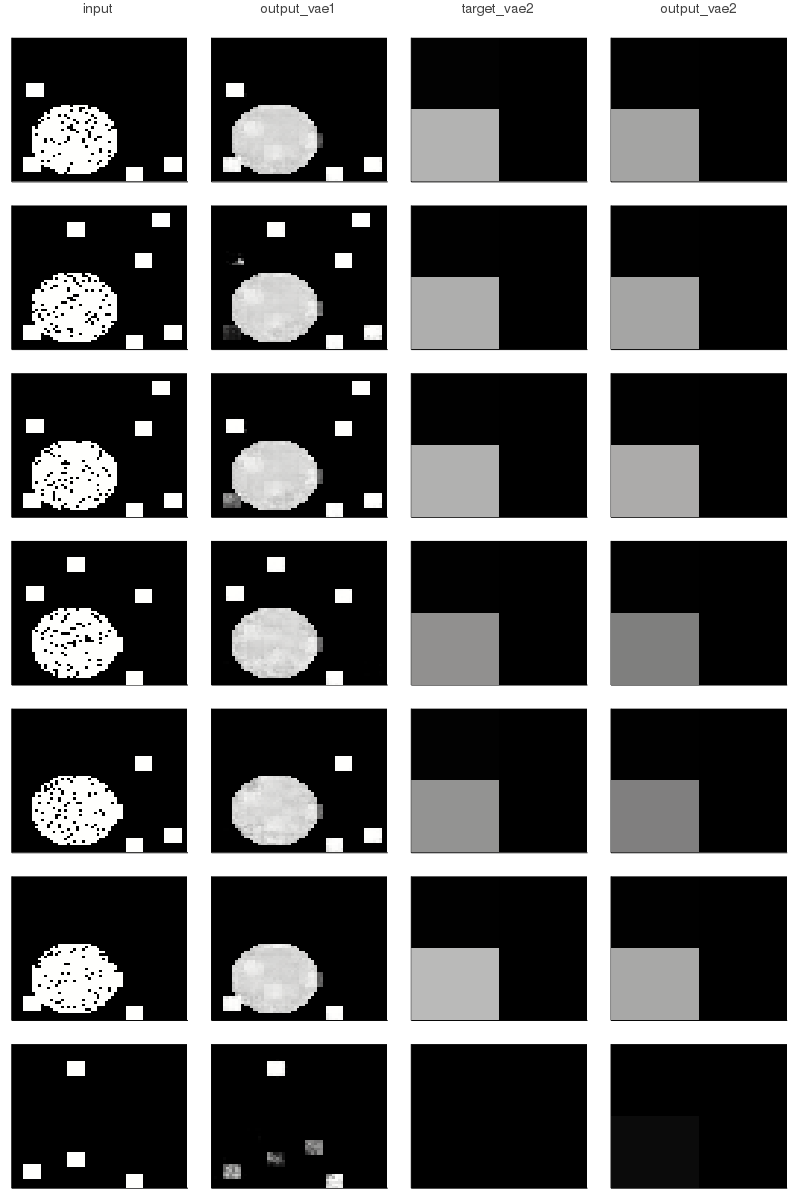
\includegraphics[width=11.5cm]{../code/plots/reconstruction1.png} 		  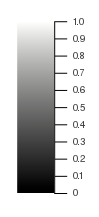
\includegraphics[width=1.5cm]{../code/plots/scale.png}
  \caption{Reconstruction plot of eight images $\mathbf{x}$ sampled from dataset $\mathbf{X}_{90}$. Each row resembles a different input image and we have columns for the input image $\mathbf{x}$, output $vae1(\mathbf{x})$, the scaled input image $g(\mathbf{x})$ and output $vae2(\mathbf{x})$.}
  \label{fig:recon1}
\end{center}
\end{figure}

\begin{figure}
\begin{center}
  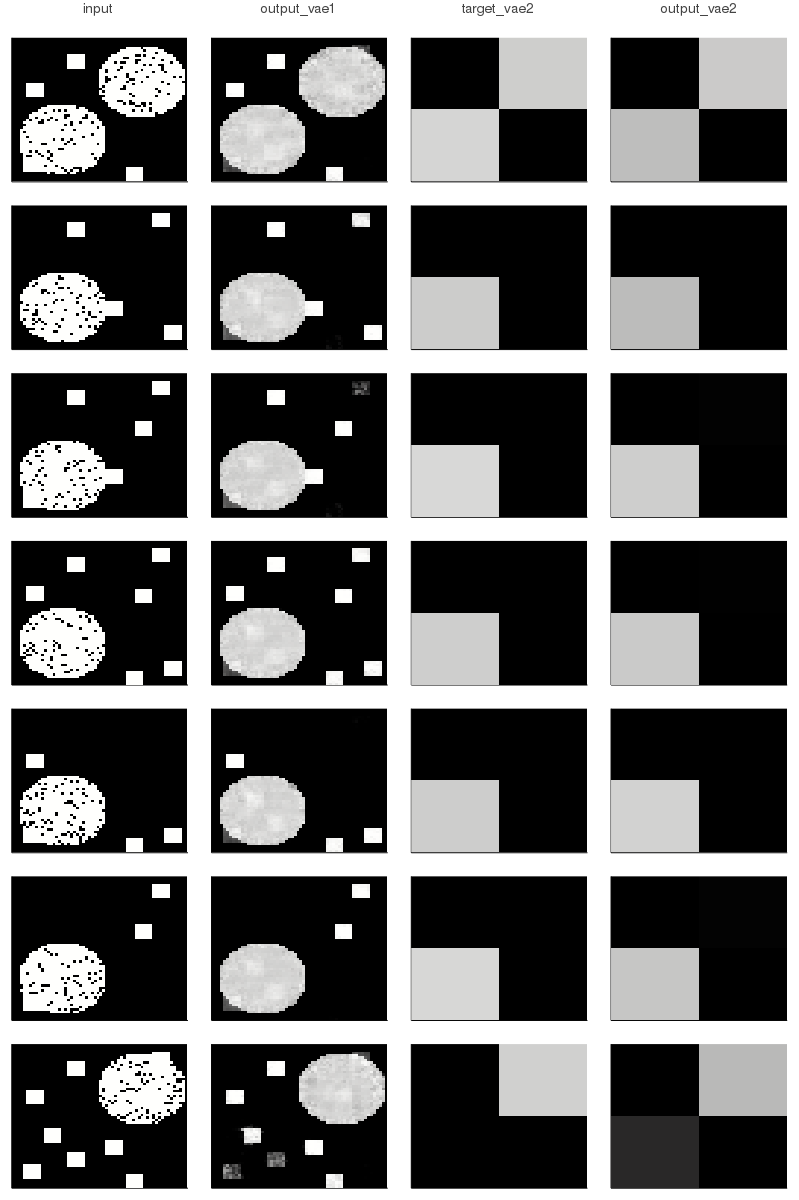
\includegraphics[width=11.5cm]{../code/plots/reconstruction3_48_55.png}
  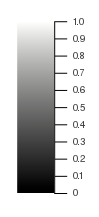
\includegraphics[width=1.5cm]{../code/plots/scale.png}
  \caption{Reconstruction plot of eight images $\mathbf{x}$ sampled from dataset $\mathbf{X}_{90, 20}$. Each row resembles a different input image and we have columns for the input image $\mathbf{x}$, output $vae1(\mathbf{x})$, the scaled input image $g(\mathbf{x})$ and output $vae2(\mathbf{x})$.}
  \label{fig:recon3}
\end{center}
\end{figure}

\begin{figure}
\begin{center}
  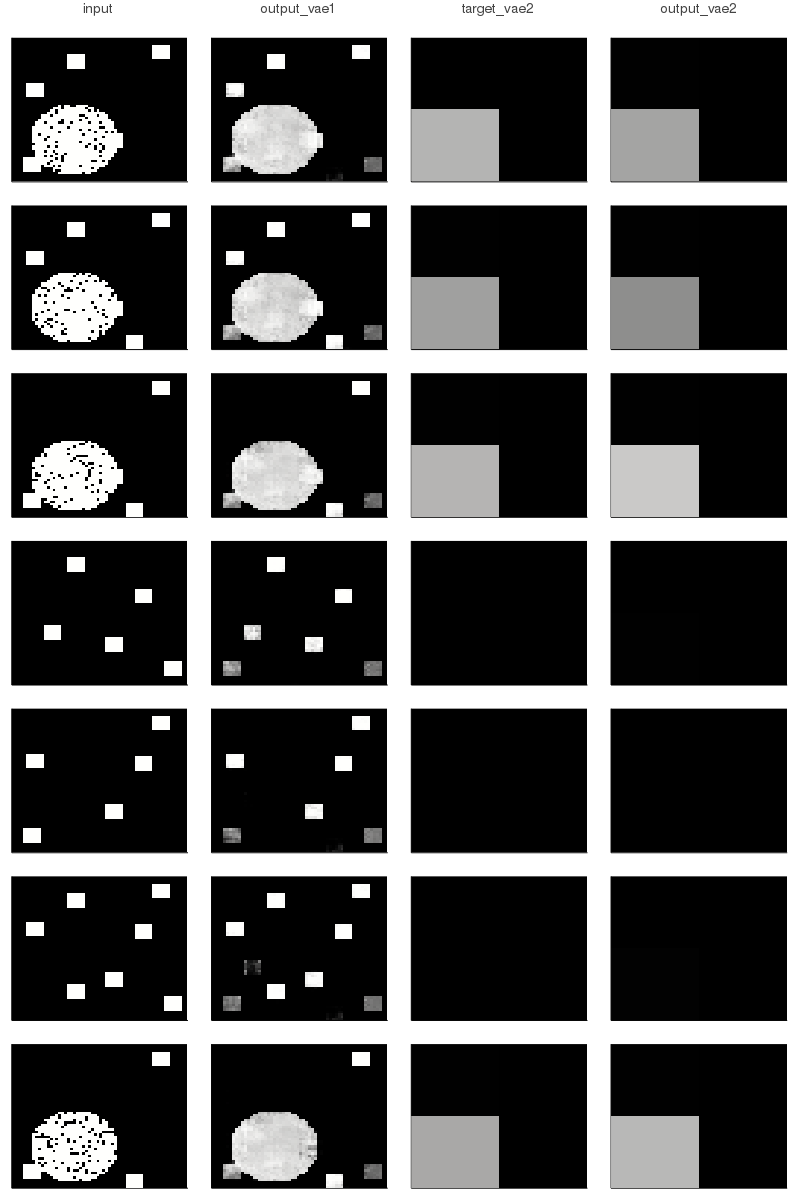
\includegraphics[width=11.5cm]{../code/plots/reconstruction2_1_8.png}
  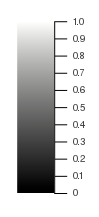
\includegraphics[width=1.5cm]{../code/plots/scale.png}
  \caption{Reconstruction plot of eight images $\mathbf{x}$ sampled from dataset $\mathbf{X}_{50}$. Each row resembles a different input image and we have columns for the input image $\mathbf{x}$, output $vae1(\mathbf{x})$, the scaled input image $g(\mathbf{x})$ and output $vae2(\mathbf{x})$.}
  \label{fig:recon2}
\end{center}
\end{figure}

\begin{figure}
\begin{center}
  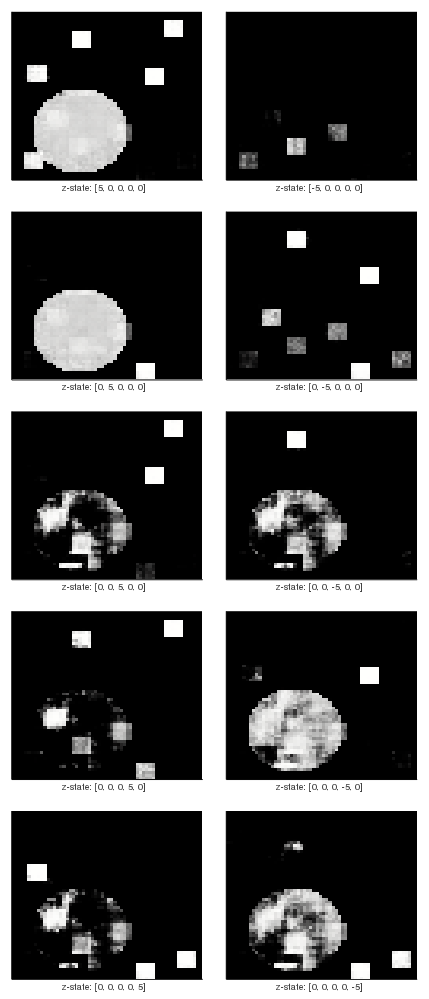
\includegraphics[width=7cm]{../code/plots/exploration1.png}
  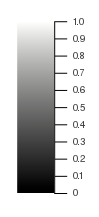
\includegraphics[width=1.5cm]{../code/plots/scale.png}
  \caption{Exploration of latent space of a dual VAE trained on dataset $\mathbf{X}_{90}$. Images show outputs of $vae1$ for different states of $\mathbf{z}_1$ and $\mathbf{z}_2$, which are annotated below the respective output in the form [$\mathbf{z}_{1, 1}$, $\mathbf{z}_{1, 2}$, $\mathbf{z}_{1, 3}$, $\mathbf{z}_{1, 4}$, $\mathbf{z}_2$].}
  \label{fig:expl1}
\end{center}
\end{figure}

\begin{figure}
\begin{center}
  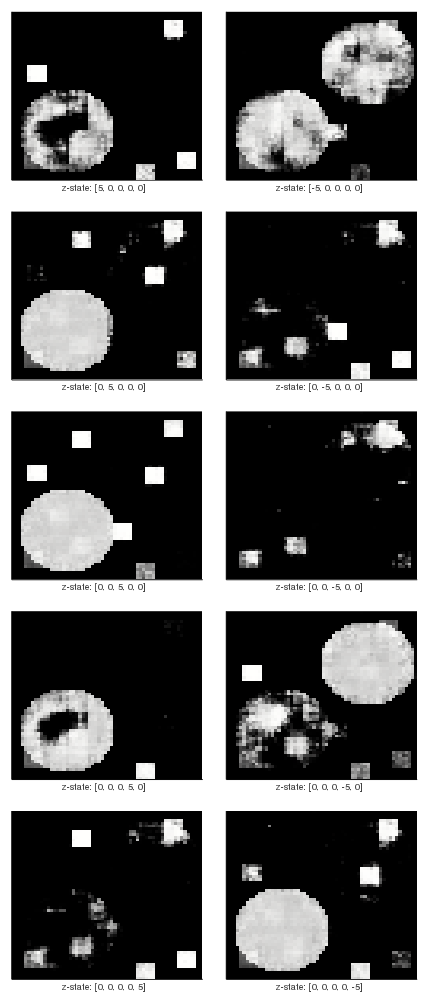
\includegraphics[width=7cm]{../code/plots/exploration3.png}
  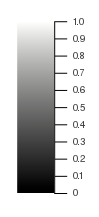
\includegraphics[width=1.5cm]{../code/plots/scale.png}
  \caption{Exploration of latent space of a dual VAE trained on dataset $\mathbf{X}_{90, 20}$. Images show outputs of $vae1$ for different states of $\mathbf{z}_1$ and $\mathbf{z}_2$, which are annotated below the respective output in the form [$\mathbf{z}_{1, 1}$, $\mathbf{z}_{1, 2}$, $\mathbf{z}_{1, 3}$, $\mathbf{z}_{1, 4}$, $\mathbf{z}_2$].}
  \label{fig:expl3}
\end{center}
\end{figure}

\begin{figure}
\begin{center}
  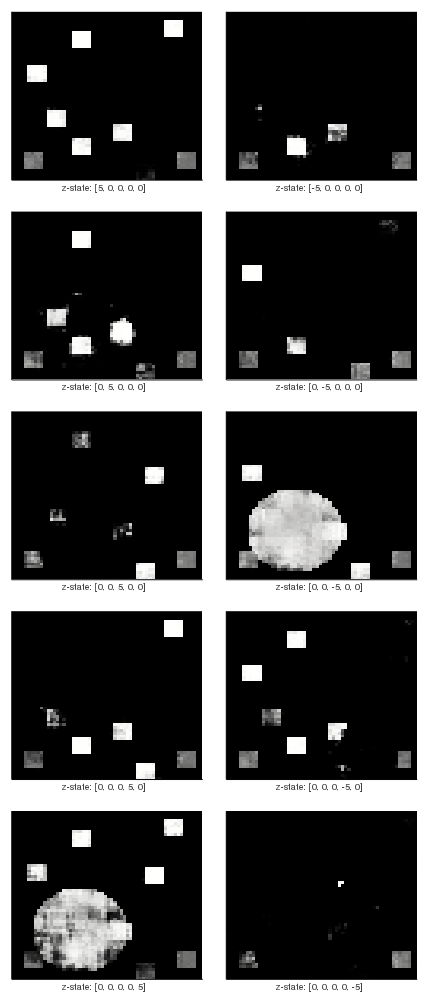
\includegraphics[width=7cm]{../code/plots/exploration2.png}
  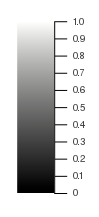
\includegraphics[width=1.5cm]{../code/plots/scale.png}
  \caption{Exploration of latent space of a dual VAE trained on dataset $\mathbf{X}_{50}$. Images show outputs of $vae1$ for different states of $\mathbf{z}_1$ and $\mathbf{z}_2$, which are annotated below the respective output in the form [$\mathbf{z}_{1, 1}$, $\mathbf{z}_{1, 2}$, $\mathbf{z}_{1, 3}$, $\mathbf{z}_{1, 4}$, $\mathbf{z}_2$].}
  \label{fig:expl2}
\end{center}
\end{figure}


\section{Discussion}
We observed, that there is a lot of differences between the results of the three scenarios we evaluated above.
The levels of the background cells were lowered in the outputs of $vae1$ across all datasets. This is a result of the noise, which forces the algorithm, that tries to maximize $\log p_{\pmb{\theta}}(\mathbf{x})$, select a lower optimal value. However we saw, that some regions within the background cells with a 90\%-activity rate had higher levels. This makes sense, as these were regions, where a foreground cell overlapped and thus neutralized the noise in case of activity embedding some of their activity into the background. Also, some of the overlapping foreground cells were decoded as active in all dimensions of the exploration plots. In this case, we argue that these cells were separated to some extend from the background cell instead of just being completely embedded into the background signal like others.

Additionaly, foreground cells that were located within 90\% active background cells, were usually reconstructed worse. Especially, if the background cell is inactive, we could see, that the reconstructed cells were distorted and showed only light activity. As some of the cells were just decoded as constantly active, we also have a high false positive rate in this case. When the background is active, we can not identify, whether the foreground cell is reconstructed as active or if we just see the background cell with embedded portions of the foreground cell.
Both problems are most probably a symptom to the fact that the background signal obstructs the foreground signal in around 9 out of 10 pictures. Hence, the data is heavily weighted towards images, where the foreground cells, that are located within the range of the activity, are poorly visible to the algorithm. As we optimize over the loss of all images, it is cheaper for the algorithm to not reconstruct these cells well and be slurry on their exact activity and by that gains headroom to reconstruct other components more correctly. Some of this activity was for example regarded as part of the background cell, like we just argued, leaving more parts of the latent space for information about other activities. Several solutions might be interesting to tackle this problem. First, we could try to upsample images with low background activity in the dataset. This would make it more expensive for the algorithm to reconstruct the cells that are obstructed incorrectly. Also, we could allow more latent dimensions adding more complexity to the model and possibly giving the algorithm the means to capture the details of obstructed foreground cells better. Also, it might be interesting to have a look at datasets with more noise in the background signal. In the binary case, this would lead to better visibility of the foreground signal within active background cells. Even more interesting might be the case of not binarizing the data. Here, different levels for background and foreground would enable even better visibility of the foreground cells obstructed by high-activity background.

Contrary to the intuition, we used when setting up the double VAE structure with a big receptive field in $vae2$, the information about background cells is spread across multiple dimensions in the latent spaces of models trained on datasets with high background activity of 90\%. One might have expected that the latent space of $vae2$, being fit to a scaled target and equipped with a big receptive field, would contain most of this activity. Reasons for this might be the choice of a less complex encoder in $vae2$ or the low dimensionality of 1 of its latent space. Also, the decoder of $vae2$ interacts with the latent variables of $vae1$. This might lead to a behavior, where the encoder of $vae1$ learns better representations to reconstruct $g(\mathbf{x})$ in $vae2$. Disabling interaction for this decoder might hence also be a promising way of pushing the VAEs to this intended behaviour.

In the scenario of a less active background cell, the behaviour of embedding information on the background signal in most parts of the latent space was not as evident. Although we saw in figure \ref{fig:recon2}, that the information on the background cell could be found in one dimension of the latent space of $vae1$ in addition to the latent space of $vae2$, the remaining parts of the space were free of background information. In this case, the double VAE setup had an even better performance at separating fore- and backround signal on the latent level. However, we also saw, that the algorithm seemed to perform worse on cells, that were not located in the areas of background signal in comparison to the other tow scenarios. At second sight, one can realize, that the number of correctly reconstructed foreground cells might in fact be higher or at least equal. In the scenarios with highly active background, the algorithm usually did not retain most information about the foreground cells within or on the edges of the background cells. As a result, the algorithm had more headroom on the level of the latent space to reconstruct cells outside of these regions better. However, in the case of a less active background, we can see in both, the scenario with 50\% backround activity and the scenario with a second 20\% active background, that the foreground cells overlapping these background cells were reconstructed better. As the background in these cases is inactive more frequently, it gets more expensive (in terms of optimizing the target) for the algorithm to ignore the activity. This probably leads to more parts of the latent space being used to retain information about these foreground cells taking away parts, that could have been used for the cells outside of background activity. We suspect, that this might be the reason for the slightly worse performance on foreground cells outside of background activity in this scenario. Again, it would be promising to do further research and comparing our reconstruction results to approaches with higher dimensionality on the latent level and more complex parameterizations of the models. 

\chapter{Conclusion}


\medskip

\begin{thebibliography}{9}

\bibitem{kingma1}
D. Kingma, M. Welling:
\textit{An Introduction to Variational Autoencoders}.
arXiv: 1906.02691 [cs.LG] (2019).

\bibitem{kingma2}
D. Kingma, M. Welling:
\textit{Auto-Encoding Variational Bayes}.
arXiv: 1312.6114v10 [stat.ML] (2014).

\bibitem{cvae}
Y. Pu et al.:
\textit{Variational Autoencoder for Deep Learning of Images, Labels and Captions}.
arXiv: 1609.08976 [stat.ML] (2016).

\bibitem{KL}
M. de Queiroz, R. Silva, R. Loschi:
\textit{Shannon Entropy and Kullback-LeiblerDivergence in Multivariate Log FundamentalSkew-Normal and Related Distributions}.
arXiv: 1408.4755 [math.ST] (2016).

\bibitem{arithmetic}
Vincent Dumoulin, Francesco Visin:
\textit{A guide to convolution arithmetic for deep learning}.
arXiv:1603.07285 [stat.ML] (2016).

\bibitem{diff}
C. Rackauckas et al.:
\textit{Universal Differential Equations for Scientific Machine Learning}.
arXiv:2001.04385v [cs.LG] (2020).

\bibitem{phot}
M. Pachitariu et al.:
\textit{Suite2p: beyond 10,000 neurons with standard two-photon microscopy}.
bioRxiv doi: 10.1101/061507d (2017).

\bibitem{stanford}
Stefano Ermon: CS 228 - Probabilistic Graphical Models.
\\\texttt{https://ermongroup.github.io/cs228-notes/}
\end{thebibliography}

\end{document}
